\documentclass[conference,a4paper,10pt]{IEEEtran}
\usepackage[T1]{fontenc}
\usepackage{cite}
\usepackage{amsmath,amssymb}
\usepackage{graphicx}
\usepackage{booktabs,tabularx,array}
\usepackage{xcolor}
\usepackage{tikz}
\usetikzlibrary{arrows.meta,positioning,fit}
\usepackage[hidelinks]{hyperref}
\usepackage{xurl}
\graphicspath{{figures/}}
\newcolumntype{Y}{>{\raggedright\arraybackslash}X}
\newcommand{\code}[1]{\texttt{\detokenize{#1}}}
\newcommand{\ind}{\mathbf{1}}
\newcommand{\reach}{\mathcal{D}}
\newcommand{\unknown}{\bot}
\definecolor{auditblue}{RGB}{26,67,107}
\definecolor{auditgold}{RGB}{168,102,24}
\interdisplaylinepenalty=2500

% Default: anonymous initial submission. main_authors.tex selects the named draft.
\newcommand{\PaperTitle}{Auditing the Blast Radius: Artifact Consistency in npm Supply-Chain Prioritization}
\newcommand{\PaperAuthors}{\IEEEauthorblockN{Anonymous Authors}}
\newcommand{\PaperPDFAuthors}{}
\newcommand{\PaperPDFSubject}{Anonymous review manuscript}
\ifdefined\IncludePaperAuthors
  % User-supplied author record. Excluded from the anonymous source package.
% Sequence follows the order supplied by the user; no email addresses were given.
\newcommand{\NamedPaperPDFAuthors}{Shahriar Hasan; Ashikul Islam}
\newcommand{\NamedPaperAuthors}{%
  \IEEEauthorblockN{Shahriar Hasan\IEEEauthorrefmark{1}, Ashikul Islam\IEEEauthorrefmark{2}}
  \IEEEauthorblockA{\IEEEauthorrefmark{1}Department of ECE, \IEEEauthorrefmark{2}Department of CSE\\
    Hajee Mohammad Danesh Science and Technology University}
}

  \renewcommand{\PaperAuthors}{\NamedPaperAuthors}
  \renewcommand{\PaperPDFAuthors}{\NamedPaperPDFAuthors}
  \renewcommand{\PaperPDFSubject}{Author-attributed manuscript draft}
\fi

\hypersetup{pdftitle={\PaperTitle},pdfauthor={\PaperPDFAuthors},pdfsubject={\PaperPDFSubject}}
% Generated by scripts/audit_artifacts.py; do not edit.
\newcommand{\PackageCount}{25,228}
\newcommand{\ReviewBudget}{253}
\newcommand{\CSVReachPositive}{20}
\newcommand{\DBReachPositive}{17,809}
\newcommand{\ScoreQueueIntersection}{65}
\newcommand{\WorkflowQueueIntersection}{20}
\newcommand{\TemporalRecords}{47}
\newcommand{\TemporalFamilies}{31}
\newcommand{\TemporalRetained}{45}
\newcommand{\TemporalEdges}{258}

% Generated field comparison.
\newcommand{\FieldComparisonRows}{%
Maintainer portfolio (max) & 22,147 & 22,147 & 0 \\
Maintainer portfolio (sum) & 22,147 & 22,147 & 0 \\
Workflow reach & 20 & 17,809 & 17,809 \\
Direct dependents & 20,331 & 20,331 & 0 \\
Workflow direct dependents & 15 & 15,017 & 15,014 \\
Transitive dependents & 20,328 & 20,328 & 0 \\
Legacy score & 22,147 & 24,502 & 17,809 \\
}


\begin{document}
\title{\PaperTitle}
\author{\PaperAuthors}
\maketitle
\begin{abstract}
Limited defensive budgets motivate prioritizing npm maintainers by downstream reach. However, reaching many repositories and reducing exposure to possible account compromises are different objectives. We study this distinction in our collected graph of \StudyPackages{} package nodes and \StudyMaintainers{} maintainer usernames. We compare five deterministic selection methods and 200 random orders across six budgets, using package and workflow-associated repository endpoints. At 100 identities, marginal coverage greedy reaches \GreedyCovered{} of \StudyWorkflowRepos{} observed workflow repositories (\GreedyCoveragePercent{}\%), versus \UnionCovered{} for exact maintainer-union ranking. Under a stipulated uniform single-account compromise model with perfect source hardening, their exposure reductions are \GreedyExposurePercent{}\% and \UnionExposurePercent{}\%, respectively. Only \GreedyExcluded{} repositories covered by greedy satisfy exclusion of every observed source identity. Preserving version continuity reduces identity--repository exposure pairs by \VersionPairsDecreasePercent{}\%, although aggregate greedy coverage remains similar. These results extend established maintainer-reach analyses with an explicit comparison of objectives and observation units. They support objective-specific prioritization and qualified structural measurements; they do not estimate incident probabilities or demonstrated control effectiveness.
\end{abstract}

\begin{IEEEkeywords}
software supply chain, npm, dependency graphs, artifact consistency, defensive prioritization, temporal validity
\end{IEEEkeywords}
\section{Introduction}
Open-source package dependencies distribute both functionality and trust. Earlier npm research established that dependency concentration and maintainer sharing create systemic points of failure~\cite{zimmermann2019}. Metadata weak-link signals also support proactive review~\cite{zahan2022}. The practical question is therefore not whether package graphs matter, but what a particular graph-derived queue measures and whether the artifacts used to construct it support that interpretation.

The repository studied here was developed around a proposal to forecast high-impact supply-chain entry points using dependency, maintainer, and public GitHub data. Its implemented collector stores npm package metadata, deps.dev dependency edges, workflow-directory observations, and imported advisories. A deterministic metric program combines maintainer portfolio size with the count of downstream packages associated with public workflows. A graph neural network is discussed in project documents but is not trained or evaluated by the available implementation.

This setting exposes a prerequisite often hidden by model-centric evaluation: a plausible score can be computed from inconsistent exports. We find that the compressed CSV and SQLite archives contain the same package population and identical maintainer and dependency metrics, while their workflow-derived metrics differ substantially. Consequently, using a shared population count or a common repository revision as a snapshot identifier is insufficient. A researcher can reproduce a reported CSV statistic faithfully while drawing conclusions inconsistent with the database in the same checkout.

We study three questions. \textbf{RQ1:} Are the supplied metric artifacts mutually consistent and reproducible from their stored graph and workflow observations? \textbf{RQ2:} How much do artifact choice, score weighting, and boundary ties change a fixed-budget defensive review queue? \textbf{RQ3:} What empirical claims remain supportable given the historical incident evidence and missing comparison population?

The resulting contribution has three parts. First, we provide a read-only audit that independently reconstructs all database metrics and compares every package across artifacts. Second, we quantify cross-artifact disagreement, queue overlap, and tie sensitivity without treating structural scores as compromise probabilities. Third, we specify a future benchmark whose time, population, outcome, and evidence requirements are explicit. Its graph model remains a hypothesis to test after those requirements are satisfied.

Our central result is a measurement result: \DBReachPositive{} of \PackageCount{} packages disagree on workflow reach, although every recomputed database metric agrees with its stored value. The two equal-weight score queues retain only \ScoreQueueIntersection{} of \ReviewBudget{} entries in common. A separate inventory of the historical companion yields \TemporalRecords{} event records across \TemporalFamilies{} family identifiers, \TemporalRetained{} retained source objects, and no eligible controls. These results support an artifact-consistency paper and a benchmark design, but cannot establish incident forecasting performance.

\section{Related Work and Novelty Boundary}
\label{sec:related}
\textbf{Structure and detection.} Zimmermann et al. study npm dependency and maintainer concentration; Zahan et al. examine metadata weak links~\cite{zimmermann2019,zahan2022}. These establish the feature families rather than their novelty here. Ohm et al. organize documented supply-chain attacks~\cite{ohm2020}. Amalfi and a recent detector benchmark evaluate released package content~\cite{sejfia2022,guo2026}. A benign release-classification label does not establish that its publisher remains uncompromised in a future horizon.

\textbf{Workflows and authority.} CI workflow characterization and ARGUS analyze security properties and injection paths beyond directory presence~\cite{koishybayev2022,muralee2023}. GitHub documents permission and privileged-trigger semantics~\cite{githubsecure}. Release-authority measurement compares predecessor release paths and reports no exact malicious-version overlap with its policy triggers in the studied cohort~\cite{santos2026}. Authority discontinuity is consequently a distinct review surface.

\textbf{Historical data and forecasting.} npm-follower preserves releases that can later disappear, and CHRONO-RESOLUTION provides release-point dependency resolution~\cite{pinckney2023,rahman2026}. SupplyTGN evaluates temporal vulnerability-risk ranking in a PyPI/OSV setting; PatchRisk studies future transitive vulnerability exposure for npm and PyPI~\cite{supplytgn2026,patchrisk2026}. These narrow any broad claim to introduce temporal package forecasting.

Table~\ref{tab:positioning} locates our empirical contribution: disagreement between co-located artifacts and its queue consequences. We claim neither a new graph architecture nor the first temporal package benchmark. The literature screen, updated on 20 October 2026, is targeted rather than systematic.
\begin{table*}[t]
\caption{Positioning against the closest research streams. Differences identify scope, not superiority.}
\label{tab:positioning}
\centering\footnotesize
\begin{tabularx}{\textwidth}{@{}>{\raggedright\arraybackslash}p{0.22\textwidth}YYY@{}}
\toprule
Work & Principal evidence & Evaluated target or artifact & Boundary for this study \\
\midrule
Small World; Weak Links~\cite{zimmermann2019,zahan2022} & Dependencies, maintainers, metadata & Concentration and metadata weaknesses & Structural descriptors already established \\
Amalfi; detector benchmark~\cite{sejfia2022,guo2026} & Released package content & Malicious-package detection & Detection labels do not define future non-events \\
CI characterization; ARGUS~\cite{koishybayev2022,muralee2023} & Workflow and action code & Configuration properties; injection paths & Directory presence is a weaker observation \\
On Good Authority~\cite{santos2026} & Predecessor release-path evidence & Authority discontinuities & Authority change and compromise differ \\
npm-follower; CHRONO-RESOLUTION~\cite{pinckney2023,rahman2026} & Archived releases; release-point resolution & Historical data resources & Graph reconstruction alone is not new \\
SupplyTGN; PatchRisk~\cite{supplytgn2026,patchrisk2026} & Temporal package/advisory evidence & Future vulnerability-risk ranking & Temporal forecasting is already studied \\
This study & Two local archives; incident-record inventory & Metric consistency, queue drift, feasibility & No fitted model or predictive benchmark result \\
\bottomrule
\end{tabularx}
\end{table*}


\section{Graph Metrics and Evidence}
\label{sec:evidence}
A dependency edge $(u,v)\in E$ points from dependent package $u$ to dependency $v$. The implementation projects stored version pairs onto package names. For observed packages $P$, its reverse transitive dependent set is
\begin{equation}
\reach(p)=\{q\in P\setminus\{p\}:q\leadsto p\}.
\end{equation}
Let $M(p)$ be the observed maintainer set and $d(m)$ its member's package portfolio size. The implemented statistics are
\begin{equation}
W_{\max}(p)=\max_{m\in M(p)}d(m),\qquad
W_{\Sigma}(p)=\sum_{m\in M(p)}d(m),
\end{equation}
with zero for an empty maintainer set. Summed portfolios can overlap; registry identities do not establish historical publication authority.

The workflow flag $h(q)$ is one if any stored version of package $q$ has a positive workflow-directory observation. Workflow reach is
\begin{equation}
B(p)=\sum_{q\in\reach(p)}h(q).
\end{equation}
It counts packages associated with directory observations, not distinct organizations, actual installations, or privileged executions. Multiple packages may map to one repository.

The field named \code{attacker_roi} stores the legacy score
\begin{equation}
S_{\alpha}(p)=\alpha\frac{W_{\max}(p)}{\max_q W_{\max}(q)}+
(1-\alpha)\frac{B(p)}{\max_q B(q)}.
\label{eq:score}
\end{equation}
Zero denominators become one. The default is $\alpha=0.5$. Neither component observes success probability or attack cost, so no attacker-return interpretation is established.

Structural exposure, workflow configuration, release-authority change, and future documented compromise are different decision targets. For a future event time $T_p$, cutoff $t$, and horizon $H$, the proposed outcome is
\begin{equation}
Y_{p,t,H}=\ind\{T_p\in(t,t+H]\}.
\end{equation}
Unknown outcomes remain unknown. A reviewed zero means no documented qualifying event under a stated surveillance protocol, not intrinsic benignness.

Each feature needs source, capture time, validity interval, fidelity, and missingness. A later registry query is not automatically an immutable historical snapshot. Likewise, a byte checksum establishes source identity rather than historical availability. We separate measured audit findings, repository-record inventories, and proposed experiments throughout.

\section{Objectives and Experimental Method}
\subsection{Maintainer Exposure Sets}
Let $M$ be the observed usernames and $P_m$ the packages linked to $m$. For an endpoint universe $U$, we construct
\begin{equation}
 E_m=\bigcup_{p\in P_m}\reach_U(p),\qquad
 A_e=\{m\in M:e\in E_m\},
\end{equation}
where $\reach_U(p)$ contains reverse-reachable endpoints of $p$, including its eligible seed endpoint. Repository endpoints are deduplicated across every package and path. We condense strongly connected components and propagate exact integer bitsets through the resulting directed acyclic graph. A separate propagation of source-identity bitsets checks the endpoint incidence relation.

\subsection{Three Quantities for the Same Selection}
For selected identities $S\subseteq M$, distinct endpoint coverage is
\begin{equation}
 C(S)=\left|\bigcup_{m\in S}E_m\right|.
\end{equation}
For repository endpoints, $C$ counts each repository reached by the selection once, regardless of how many selected accounts reach it.

To model source-account hardening, suppose exactly one observed username is selected uniformly as a hypothetical compromise origin. Assume a perfect control prevents that origin when selected, while all other scenarios and graph paths remain unchanged. The proportional reduction in expected endpoint count is then
\begin{equation}
 H(S)=\frac{\sum_{m\in S}|E_m|}{\sum_{m\in M}|E_m|}.
 \label{eq:exposure}
\end{equation}
The uniform prior cancels in the ratio; no compromise probabilities are fitted. Because the numerator adds account-specific reach, sorting by exact $|E_m|$ maximizes $H$ at equal costs. A repository reached by two selected accounts contributes to both scenarios. Selecting one account leaves the other account's paths intact.

Finally, we count endpoints for which every observed source has been selected:
\begin{equation}
 P(S)=\sum_{e\in U}\ind[A_e\ne\varnothing\ \land\ A_e\subseteq S].
 \label{eq:exclusion}
\end{equation}
We call this \emph{all-source exclusion}. Requiring a nonempty $A_e$ prevents credit for missing source evidence. The difference $C(S)-P(S)$ counts covered endpoints with at least one unselected source. This interpretation depends on the assumed control and observed source sets.

\begin{figure}[t]
\centering
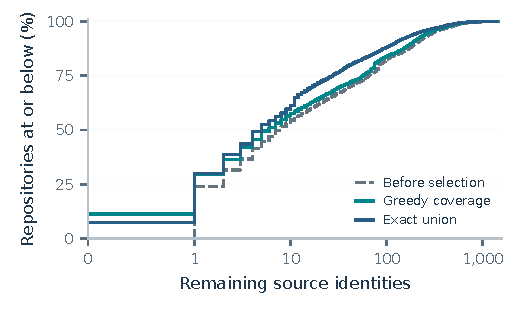
\includegraphics[width=\columnwidth]{source_multiplicity_compact.pdf}
\caption{Remaining sources at budget 100 over 7,158 source-reachable repositories. Zero remaining sources identify all-source exclusions. The horizontal scale is logarithmic above one.}
\label{fig:sources}
\end{figure}

\subsection{Selection Rules and Budget Grid}
We compare portfolio size, summed per-package reach, maximum per-package reach, exact portfolio-union reach, and greedy maximum marginal coverage. The sum baseline double-counts overlap within a portfolio. Greedy repeatedly adds the identity contributing the most newly covered endpoints. Coverage is monotone submodular, so this established method has the standard $1-1/e$ lower bound relative to optimal coverage~\cite{nemhauser1978}; that guarantee does not apply to $H$ or $P$. The additional exclusion-oriented heuristic has no global optimality guarantee.

Each rule produces nested selections at budgets $1,5,10,25,50,100$, with equal account costs and ascending usernames to break ties. The random baseline uses 200 seeded uniform orders without replacement; each order is reused across endpoint universes. Hypergeometric probabilities supply exact expectations from source multiplicities. Central 95\% simulation ranges describe variation between selections on this graph. They provide no population confidence interval for npm. We saved an exploratory analysis plan before execution, without external preregistration.

% Declare the wide budget plot early so it can float beside the results.
\begin{figure*}[t]
\centering
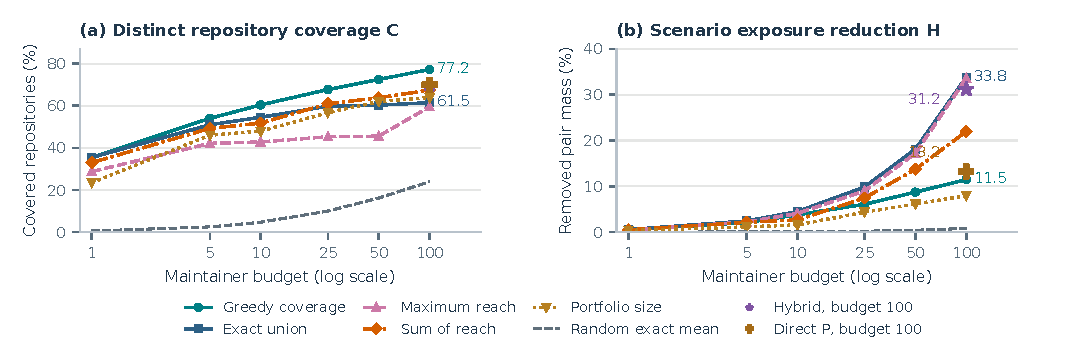
\includegraphics[width=\textwidth]{objective_tradeoff.pdf}
\caption{Workflow-repository coverage and conditional exposure reduction favor different selections. Lines connect the six evaluated budgets. The random curve is the exact expectation; stars and plus markers show the two additional budget-100 sensitivities.}
\label{fig:budget}
\end{figure*}

\subsection{Reproducibility and Checks}
The read-only Python implementation records hashes, seeds, environment, and definitions. Breadth-first searches independently verify 288 roots and all 25,228 stored package transitive counts; dual incidence, union bounds, nested curves, and $P\le C$ are checked. Tests cover cycles, version splicing, and 675 roots in 60 seeded small graphs. The grid contains 150 deterministic and 6,000 random budget rows across five endpoint/visibility definitions. No package payload is executed.

Three isolated full reruns reproduce aggregate results byte for byte. On Linux x86-64 with Python 3.14.8, mean wall time is 39.50 s (sample SD 0.98 s), with maximum peak RSS 1,038.4 MiB. These include extraction, baselines, sensitivities, and serialization; uncontrolled caches preclude online-cost inference.


\subsection{Additional Structural Sensitivities}
At budget 100, a hybrid greedily maximizes marginal gain of $J_\alpha(S)=\alpha C(S)/|U|+(1-\alpha)H(S)$ at $\alpha=0.50$. A separate heuristic lexicographically prioritizes immediately completed source sets, fractional remaining-source contributions, marginal coverage, and username order. Candidates come from endpoints with one to ten remaining sources, falling back to all unselected identities.

To distinguish the earlier residual threshold from strict exclusion, define $R_+=\{e:A_e\ne\varnothing\}$ and
\begin{equation}
 T_k(S)=|\{e\in R_+:|A_e\setminus S|<k\}|,\quad
 \Delta T_k=T_k(S)-T_k(\varnothing).
\end{equation}
$T_k$ is a residual-source count, not an enforced review quorum. The strict variant $P_k^{\rm strict}$ counts only endpoints with zero remaining sources or with $|A_e|\ge k$ and fewer than $k$ remaining sources. It has zero baseline; all 13 source-free endpoints are excluded. Uniform efficacy sensitivity $H_\eta=\eta H$ scales the stipulated exposure reduction without estimating a bypass rate.

\section{Results}
\subsection{RQ1: Coverage and Exposure Favor Different Selections}
Table~\ref{tab:methods} reports workflow-repository outcomes at 100 identities (0.819\% of usernames). Greedy covers \GreedyCovered{} repositories (\GreedyCoveragePercent{}\%), versus \UnionCovered{} (61.5\%) for exact union: a descriptive difference of $\Delta C = +1{,}131$ repositories (+25.7\%). Exact union instead removes \UnionExposurePercent{}\% of stipulated exposure, versus \GreedyExposurePercent{}\% for greedy ($\Delta H = -22.30$ percentage points; $\Delta P = +266$). Its $H$ advantage follows analytically; the experiment quantifies the resulting coverage tradeoff. Maximum reach nears this $H$ but covers fewer repositories.

\begin{table}[t]
\centering
\caption{Workflow-repository results at 100 identities. $C$: distinct coverage; $H$: conditional scenario exposure reduction; $P$: all-source exclusion. Random values are 200-order means.}
\label{tab:methods}
\small
\begin{tabular}{lrrrr}
\toprule
Selection & $C$ & $C$ (\%) & $H$ (\%) & $P$\\
\midrule
\ResearchMethodRows
\bottomrule
\end{tabular}
\end{table}

Figure~\ref{fig:budget} compares all six budgets. At 100, the 200 random orders give mean coverage 1,680.6 (sample SD 530.7; Monte Carlo standard error $\text{MCSE}_C=37.5$). Their mean $H$ is 0.80\% (SD 0.373 pp; $\text{MCSE}_H=0.026$ pp). The exact expectations are $E[C]=1{,}716.8$ and $E[H]=100/12{,}217=0.819\%$. These differences arise between finite random selections on the retained graph.



\subsection{RQ2: Covered Endpoints Retain Other Sources}
Figure~\ref{fig:sources} shows source multiplicities; Fig.~\ref{fig:partition} partitions source-reachable repositories at budget 100. Of the 5,538 repositories covered by greedy, only 800 meet all-source exclusion; 4,738 remain reachable from an unselected identity. Across the 7,158 repositories with nonempty observed source sets, 6,358 retain such a source. Exact-union ranking excludes every observed source for 534 repositories. Neither baseline optimizes $P$.

\begin{figure}[t]
\centering
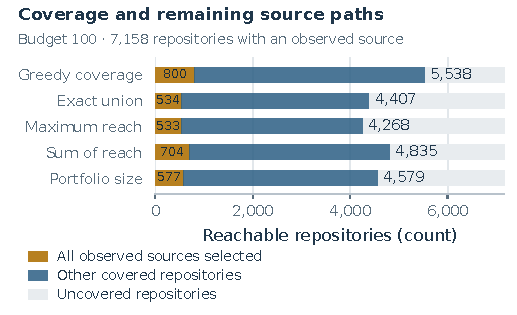
\includegraphics[width=\columnwidth]{coverage_partition.pdf}
\caption{Repository source-set partition at budget 100. Segment labels give all-source exclusion, covered residual exposure, and uncovered counts. Bars exclude 13 repositories without observed sources. Blue segments remain reachable through unselected identities.}
\label{fig:partition}
\end{figure}

Overlap explains why coverage and account-origin exposure diverge. At 100 identities, $1-C(S)/\sum_{m\in S}|E_m|$ is 89.57\% for greedy and 97.18\% for exact union. In the retained graph, \texttt{qix} is linked to \QixPortfolio{} packages and ranks \#2,298 by portfolio size. Its \QixNameReach{} workflow-repository endpoints place it \#\QixUnionRank{} by exact union; version continuity gives \QixVersionReach{} and rank \#\QixVersionRank{}. Of its name-graph endpoints, \QixOutsideSindresorhus{} lie outside \texttt{sindresorhus}'s reach. Greedy selects \texttt{sindresorhus} first and \texttt{tootallnate} eighth, but omits \texttt{qix} from its first 100 selections. Its endpoints therefore retain that unselected source. These are snapshot associations, not historical forecasts.

\subsection{RQ3: Representation Changes Exposure Mass}
Preserving version continuity changes downstream closures for \ChangedRoots{} of 25,228 package roots and removes 1,273,291 ordered root--dependent pairs introduced by package projection. Maintainer workflow-repository unions change for 2,582 usernames. Total identity--repository pairs fall from 462,170 to 266,016, a \VersionPairsDecreasePercent{}\% decrease. This is representational sensitivity, not an estimate of false exploit paths in actual installations.

At 100 identities, selecting and evaluating greedy on the version graph covers 5,516 repositories, with $H=13.10\%$ and $P=817$. Exact-union ranking gives $C=4,479$, $H=40.59\%$, and $P=527$. Evaluating the package-selected greedy identities on that version graph yields $C=5,491$. Aggregate coverage remains similar at this budget, while additive exposure mass is substantially representation-dependent (Fig.~\ref{fig:representation}).

\begin{figure}[t]
\centering
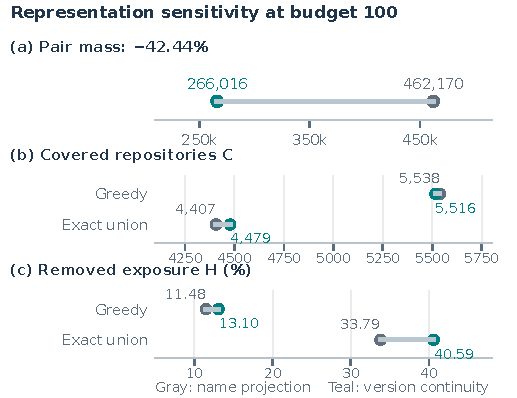
\includegraphics[width=\columnwidth]{representation_detail.pdf}
\caption{Version continuity changes pair mass while aggregate coverage remains similar. The lower panels report coverage and exposure, selecting and evaluating within each representation at budget 100. Both graphs remain observed unions.}
\label{fig:representation}
\end{figure}

Repository deduplication affects decisions. Selecting greedy for all-package coverage, then evaluating repository endpoints, covers 5,308 repositories; selecting for workflow-package coverage gives 5,315. Direct repository selection gives 5,538. Depth ablation gives 5,255 when selection uses portfolio endpoints alone and 5,488 with one-hop evidence, both evaluated against full reach. Endpoint units and depth therefore matter with the final evaluation denominator held fixed.

\section{Robustness and Research Implications}
\subsection{Observation and Selection Sensitivities}
We exclude 60 positive observations whose stored repository key disagrees with a lexical parse of the source URL, reducing the endpoint universe by 24 repositories (7,171 to 7,147); greedy at 100 covers 5,524, with $P=799$. We do not transfer workflow flags without reacquisition. This check addresses a specific mapping defect and cannot certify remaining remote associations.

Removing all bundled-context nodes leaves every workflow-repository source set unchanged, including all 462,170 identity--repository pairs. Consequently, primary repository $C$, $H$, and $P$ are identical for any fixed selection. Workflow-package incidence changes by 28 pairs for one endpoint, which repository deduplication absorbs; contextual nodes should therefore not be assumed irrelevant to every endpoint definition.

Reversing tie order yields $C=5{,}537$ and $P=793$. Excluding the 1, 5, or 10 largest portfolios gives coverage of 5,522, 5,149, and 5,076. Grouping equal stored email hashes as a hypothetical control unit yields 12,147 groups with greedy coverage at 5,538. These tests reflect eligibility sensitivity rather than verified credential control.

\subsection{From Structural Reach to Outcome Research}
Our findings suggest distinct uses for the quantities. A team seeking broad review coverage can use $C$; the stipulated fixed-prior account-hardening decision uses $H$. Complete modeled source exclusion requires $P$ and may demand complementary selections. Actual budgets also depend on control cost, feasibility, account-specific probabilities, publishing permissions, and adversary adaptation. Our equal-cost fixed-prior experiment does not observe these. Workflow association alone cannot establish credential-harvesting return or a control's causal effect.

We completed prospective acquisition groundwork by sampling 100 identifiers uniformly without replacement from our 25,228-name frame (seed 20261020, frozen before requests). Metadata were captured for 90; eight HTTP 405 responses involve bundled identifiers, while two return HTTP 404. The feature cutoff is 20 October 2026, 00:48:38 Asia/Dhaka, with a 90-day horizon ending 18 January 2027. All 100 outcomes remain pending. This pilot demonstrates feasibility; its size does not establish event yield or predictive power.

Future compromise evaluation must fix surveillance sources, reporting delays, censoring, and family-grouped splits before examining outcomes. Unreported packages remain unlabeled rather than certified benign. Contemporary metadata cannot be retroactively assigned to earlier attacks. We report no trained forecast, accuracy, or empirical compromise probability from this pilot.

\section{Threats to Validity and Research Ethics}
\subsection{Construct and Internal Validity}
Structural reach is conditional on the observed graph. Package projection removes version constraints; public workflow-directory observations do not establish execution, permissions, or installations. Maintainer usernames need not correspond one-to-one with current publishers or organizations. The legacy score's normalization is sample-dependent, and CSV rounding can enlarge score ties. These limitations apply even when recomputation succeeds.

Our audit localizes cross-artifact differences but does not reconstruct their cause. Differences could arise from workflow collection timing, export timing, or another undocumented process. We do not diagnose a specific fault without capture records. Matching database recomputation validates consistency with the stored inputs and formula, not correctness or completeness of the original collection.

The queue comparison uses a registered-in-code one-percent budget and an explicit name rule. Other budgets, normalization schemes, and tie policies can yield different values. The reported weight sweep is descriptive rather than a robustness guarantee. Deterministic totals over a finite artifact do not require sampling confidence intervals; they cannot be generalized to the full npm ecosystem using the same rationale.

\subsection{External and Temporal Validity}
The collector's high-impact seeding and recursive discovery overrepresent some parts of npm. Missing repositories and unchecked workflow states are not evidence of low risk. Several package observations can share a repository or maintainer, and related campaigns further reduce independent units. No ecosystem-wide compromise rate follows from these data.

The temporal companion is inventoried from existing CSVs. We do not independently re-adjudicate all 47 incident records, verify retained raw response bytes, or reproduce historical workflow snapshots. Pre-event source selection from a later registry response does not guarantee historical immutability. Source deletion and availability may depend on maliciousness; surviving records can therefore induce selection bias. npm-follower motivates retention at publication time, but its reported coverage is not assumed to cover our incident set~\cite{pinckney2023}.

The novelty screen covers selected primary papers and documentation available by 20 October 2026. It is not a systematic literature review and cannot establish an exhaustive absence of similar studies. Recent forecasting and authority-measurement work is explicitly acknowledged rather than excluded through a narrow terminology choice.

\subsection{Data Handling and Reproducibility}
The audit works offline on supplied archives, opens SQLite read-only, and publishes aggregate output rather than new lists labeling maintainers or packages as malicious. It neither installs suspicious packages nor collects secrets. The source repository retains its original artifacts; manuscript-specific results record their full hashes. The paper package includes source, figures, generated numeric tables, and rebuild instructions. Raw databases are referenced rather than duplicated in the writing package.

Author identities and affiliations are intentionally left for the actual contributors to supply. The document is a research draft, with a measured audit and a proposed benchmark; it does not assert peer review, acceptance, funding, institutional approval, or completed predictive validation.

\section{Conclusion}
At 100 identities, greedy covers 5,538 workflow repositories but excludes all observed sources for only 800; exact union yields greater conditional exposure reduction. Version continuity reduces exposure pairs by 42.44\%. Hybrid and exclusion-oriented selections illustrate additional tradeoffs; threshold increments and efficacy multipliers remain hypothetical sensitivities. Version-aware inventory and release-age delays~\cite{he2025} complement account controls, but we establish no optimal 3-to-7 day cooldown. Railway's deployment pause motivates build-independent revocation and recovery paths~\cite{railwaydisclosure2026}; their effectiveness is not measured here. Pending prospective outcomes support no forecasting claim.

\section*{Acknowledgment}
A large language model assisted literature discovery, audit-code development, manuscript drafting, and editing. Numerical results were recomputed from the supplied artifacts. Human authors must review and approve the sources, code, interpretations, and disclosure before submission.

\bibliographystyle{IEEEtran}
\bibliography{bibliography/references}
\end{document}
